\section{Theory}
\label{sec:Theory}
\subsection{The Sagnac Interferometer}
\label{sec:The_Sagnac_Interferometer}
A Sagnac interferometer is a device built out of multiple mirrors and a polarising beam splitter cube (PBSC). Its purpose is to split a laser beam entering the interferometer into two beams, which can the be redirected over different path. A sketch of the device can be seen in \autoref{fig:interferometer}.\\
To split the beam, it first goes through the PBSC at a $45$ degree angle to the beam. This reflects s-polarised light, while transmitting p-polarised light. The beams then get reflected thrice via multiple mirrors to reenter the PBSC. A portion of each of these beams is then transmitted/reflected into the output area, as shown in \autoref{fig:interferometer}.\\
\begin{figure}
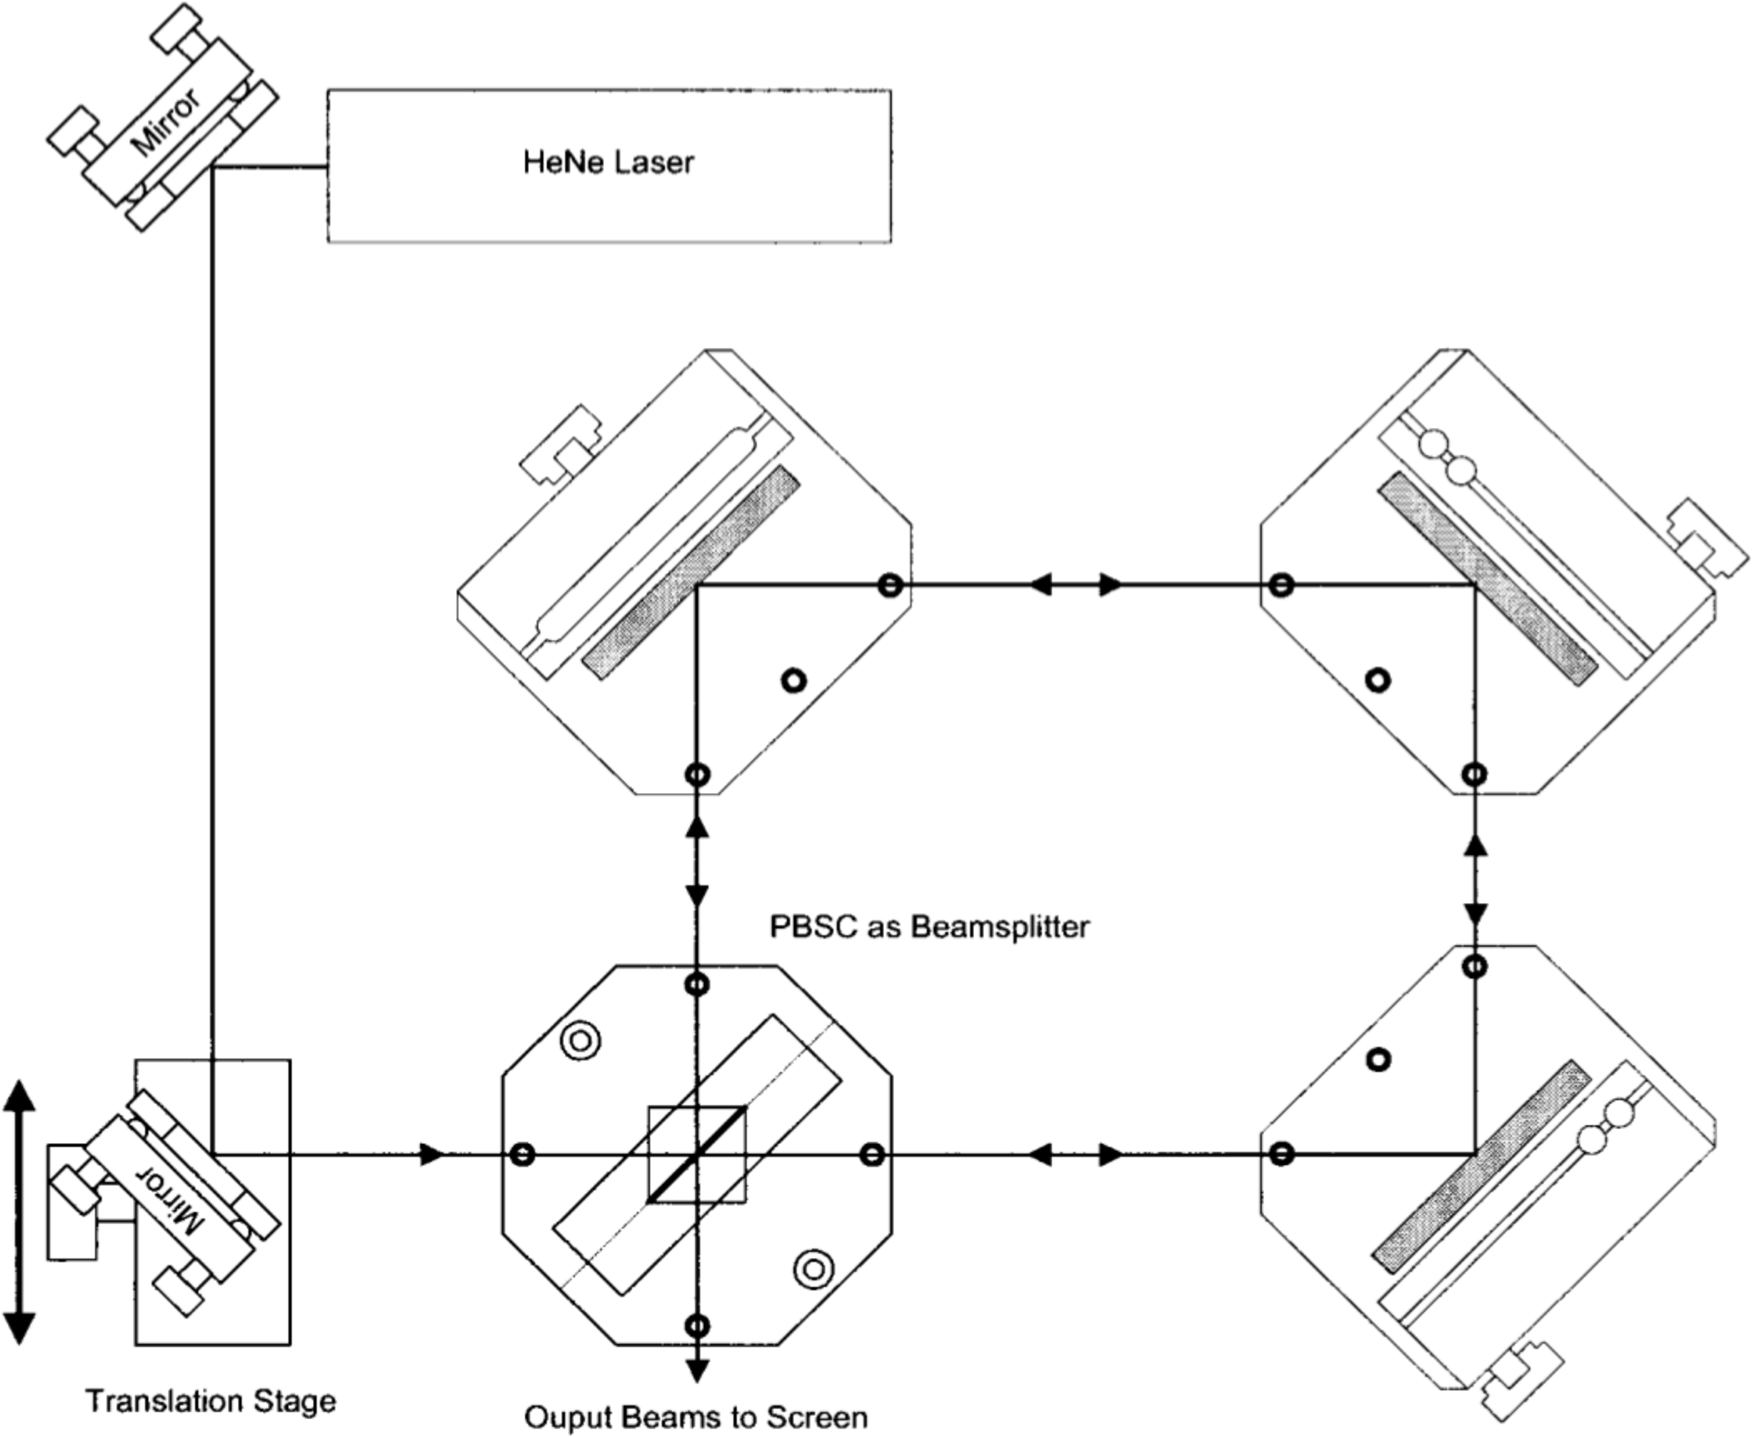
\includegraphics[width=\linewidth]{./figures/aufbau.pdf}
\caption{The Sagnac Interferometer}
\label{fig:interferometer}
\end{figure}
However if the interferometer is perfectly adjusted, the resulting beams will overlap at all stages of the interferometer. To manipulate each beam individually, it is necessary to separate their superposition. To do so the laser, or in this case the mirror between the laser and the mirror, has to be moved in the direction that is shown by the arrow in the picture. Doing so results in the two beams following different paths after entering the PBSC. During this stage, one of the beams can be sent through a medium, making it possible to measure the medium's refraction index.
\\
An important quantity for interferometers is the contrast. The name is self-explanatory: Just like in the case of colours, where the contrast between two colours is highest if they are opposite to each other (for example black and white) and lowest if both colours are the same, the contrast in an interference picture is defined as 
\begin{aquation}
  K &= \frac{I_\text{max}-I_\text{min}}{I_\text{max} + I_\text{min}} \tc
  \label{eq:contrast}
\end{aquation}
with minimal and maximal intensities $I_\text{min}$ and $I_\text{max}$.\\
The closer the contrast is to $1$, the better it is. On the other hand, it is worse the lower it is. The ideal contrast therefore occurs for $I_\text{min}=0$, while the worst case is that there are no minima/maxima, meaning that $I_\text{min}=I_\text{max}$.\\
In this experiment, the contrast will be measured dependent on the phase angle of a polarisation filter that has been positioned in the beam's path. For this, the contrast takes the form 
\begin{aquation}
K &= A|\sin(2\varphi + \delta)| \tp
\end{aquation}

\subsection{Interference}
Before going through interference itself, some general remarks on a wave's intensity should be made.\\
To get the intensity of any wave (which is what is measured buy a photo diode), the formula 
\begin{aquation}
  I \coloneqq \varepsilon_0 c \langle | \vec{E}\left(z, t\right) |^2 \rangle
\end{aquation}
has to be applied. Here, 
\begin{aquation}
  \langle f(t) \rangle &\coloneqq \frac{1}{T}\int_{t_0}^{t_0 + T} f(t)
\end{aquation}
is the time average of a function $f(t)$ with period $T$, while 
\begin{aquation}
  \vec{E} &\coloneqq \text{Re}\left(\left[E_x \vec{e}_x + E_y \vec{e}_y e^{i \delta}\right] e^{i k z - i \omega t}\right) \\
  &= E_x \vec{e}_x \cos(k x - \omega t) + E_y \vec{e}_y \cos(k y - \omega t + \delta)
\end{aquation}
is the wave's electric field component, with any phase $\delta$, which determines a wave's initial polarisation (ellipticity and its special cases). This phasee is a relative phase between the $x$- and $y$-part of a wave's electric field. In other conventions, the above expression might occur in a symmetrised form, assigning a phase $\delta_{x,y}$ to each of the respective electric field's components.\\
Since the time average of any squared cosine is $\frac{1}{2}$, the intensity becomes 
\begin{aquation}
  \label{eq:single_beam}
  I &= \varepsilon_0 c \frac{E_0^2}{2}
\end{aquation}
with $E_0^2 \coloneqq E_x^2 + E_y^2$.\\
But interference occurs only when two coherent beams with a relative phase shift $\varphi$ overlap, since the total electric field of the combined beam is the superposition of the single beams. Mathematically, this makes the intensity
\begin{aquation}
  I &= \varepsilon_0 c \langle | \vec{E}_1\left(z, t\right) + \vec{E}_2\left(z, t, \varphi\right) |^2 \rangle \tp
\end{aquation}
Factorising the absolute value there are two field squares of the type $\vec{E}_i^2$ occuring, which leads to two terms like the one derived earlier for each single beam. But in addition to this, there is a mixed term between the two waves, which is called an \textit{interference term} for a reason.\\
Using the fact that the time average does not care about the occurence of a total phase $\delta$ in both cosines in the cosine-product, the total mixed amplitude then reads 
\begin{aquation}
  \label{eq:double_beam}
  I &= \varepsilon_0 c \left( \varepsilon_0 c \langle | \vec{E}_2\left(z, t\right) |^2 \rangle + \langle | \vec{E}_2\left(z, t, \varphi\right) |^2 \rangle + 2 \langle \vec{E}_1\left(z, t\right) \cdot \vec{E}_2\left(z, t, \varphi\right) \rangle \right) \\
  &= \varepsilon_0 c \left(\frac{E_1^2 + E_2^2}{2} + \left(E_{1 x} E_{2 x} + E_{1 y} E_{2 y}\right) \cos\left(\phi\right)\right) \tp
\end{aquation}
This is the general formula for an arbitrary beam split and relative phase (since $E_{1,2}^0$ and $\varphi$ can be chosen arbitrarily).\\
To become more specific, the special case of a $50/50$  beam split (meaning $\vec{E}_1^0 = \vec{E}_2^0 \eqqcolon \vec{E}_\text{split}$, $\varphi=0$) without a relative phase shift will be considered. In this case, using \autoref{eq:single_beam} for the beam before splitting and \autoref{eq:double_beam} for the beams after splitting, demanding that the total intensity is the same in both instances, it follows that 
\begin{aquation}
  \vec{E}_\text{split} &= \frac{\vec{E}_0}{\sqrt{2}} \tp
\end{aquation}
It does not matter if there is going to be a phase shift later in the beam - at the splitting point, this equation of continuity always holds.
\begin{aquation}
  I &= \varepsilon_0 c \left(\frac{E_0^2}{2} + \frac{E_0^2}{2} \cos\left( \varphi \right) \right) \tp
\end{aquation}
For this phase-dependent intensity, the minimal/maximal intensity occur at the cosine's extrema. The maximum lies at $\varphi=0$, while the minimum is at $\varphi=\pi$, yielding
\begin{aquation}
  I_\text{max} &= E_0 \tc \\
  I_\text{min} &= 0 \tc
\end{aquation}
which is exactly what is expected for these cases.\\
It can also be noted that this is completely independent of the $z$-coordinate, since it is integrated out in the process of taking the time average. However, the equation would become space dependent if the beams are not perfectly aligned, since in that case the non-$z$-dependent part of the wave would not vanish during time averaging. This effect is crucial to understand because during adjustment, a tilt like this will result in interference fringes after the beams have been 'aligned', which have to be removed to reach true alignment as the final step of adjustment.

\subsection{The Refraction Index}
The refraction index of a medium is a measure for how fast light travels inside that medium. It is manifest in the dispersion relation inside the medium, effectively scaling the speed of light's vacuum value. This means that 
\begin{aquation}
  n &= \frac{c_\text{med}}{c_\text{vac}} \tp 
\end{aquation}
Plugging this into the vacuum dispersion relation, the resulting refraction index inside the medium, depending on the wave number inside the medium, is
\begin{aquation}
  n &= \frac{\lambda_\text{vac} k}{2\pi} \tp
\end{aquation}
In any medium with refractive index $n$, the phase shift that occurs when a beam has moved a distance $L$ is 
\begin{aquation}
  \phi &= \frac{2\pi}{\lambda} n L \tp
\end{aquation}
Both beams will have such a phase shift after moving through the distance $L$, and the phase shift will be different since the media are different. But their relative phase shift is just the difference between the total phases. For this reason, the phase shift caused by one beam traveling through a medium of length $L$ while the other travels through a medium with $n \approx 1$ (like the vacuum or air) will be 
\begin{aquation}
  \label{eq:phase_shift}
  \varphi &= \frac{2\pi}{\lambda} (n - 1) L \tp
\end{aquation}
The number of interference maxima that occurs due to a phase shift is 
\begin{aquation}
  N &= \frac{\varphi}{2\pi} \tp
\end{aquation}
Plugging \autoref{eq:phase_shift} into this equation yields 
\begin{aquation}
  n &= 1 + \frac{N\lambda}{L} \tc
\end{aquation}
which makes it possible to determine the refractive index when $L$, $\lambda$ and $N$ are known.

\subsubsection{Gaseous Medium}
To measure this index, one of the beam is lead through a gas cell. The difference in the speed of light inside the cell yields a phase difference 
\begin{aquation}
  \Delta \varphi &= \frac{2 \pi L}{\lambda_\text{vac}}\Delta n
\end{aquation}
between the two beams, which results in them interfering with each other after being reunited. The number of maxima of interference is proportional to the phase difference. It is 
\begin{aquation}
  M &= \frac{\Delta \varphi}{2 \pi} \tp
  \label{eq:interference_maxima}
\end{aquation}
The Lorentz-Lorenz equation 
\begin{aquation}
  \frac{n^2-1}{n^2+1} &= \frac{N \alpha}{3\epsilon_0}
  \label{eq:Lorentz-Lorenz}
\end{aquation}
with the particle density $N$.\\
Since the refraction index of a gas is $\approx 1$, it can be expanded, yielding
\begin{aquation}
  n &= \approx \sqrt{1 + \frac{3 A p}{R T}} \tp
\end{aquation}
This means that the refraction index can be measured by varying the gas's pressure and/or temperature.

\subsubsection{Solid Medium}
\begin{figure}
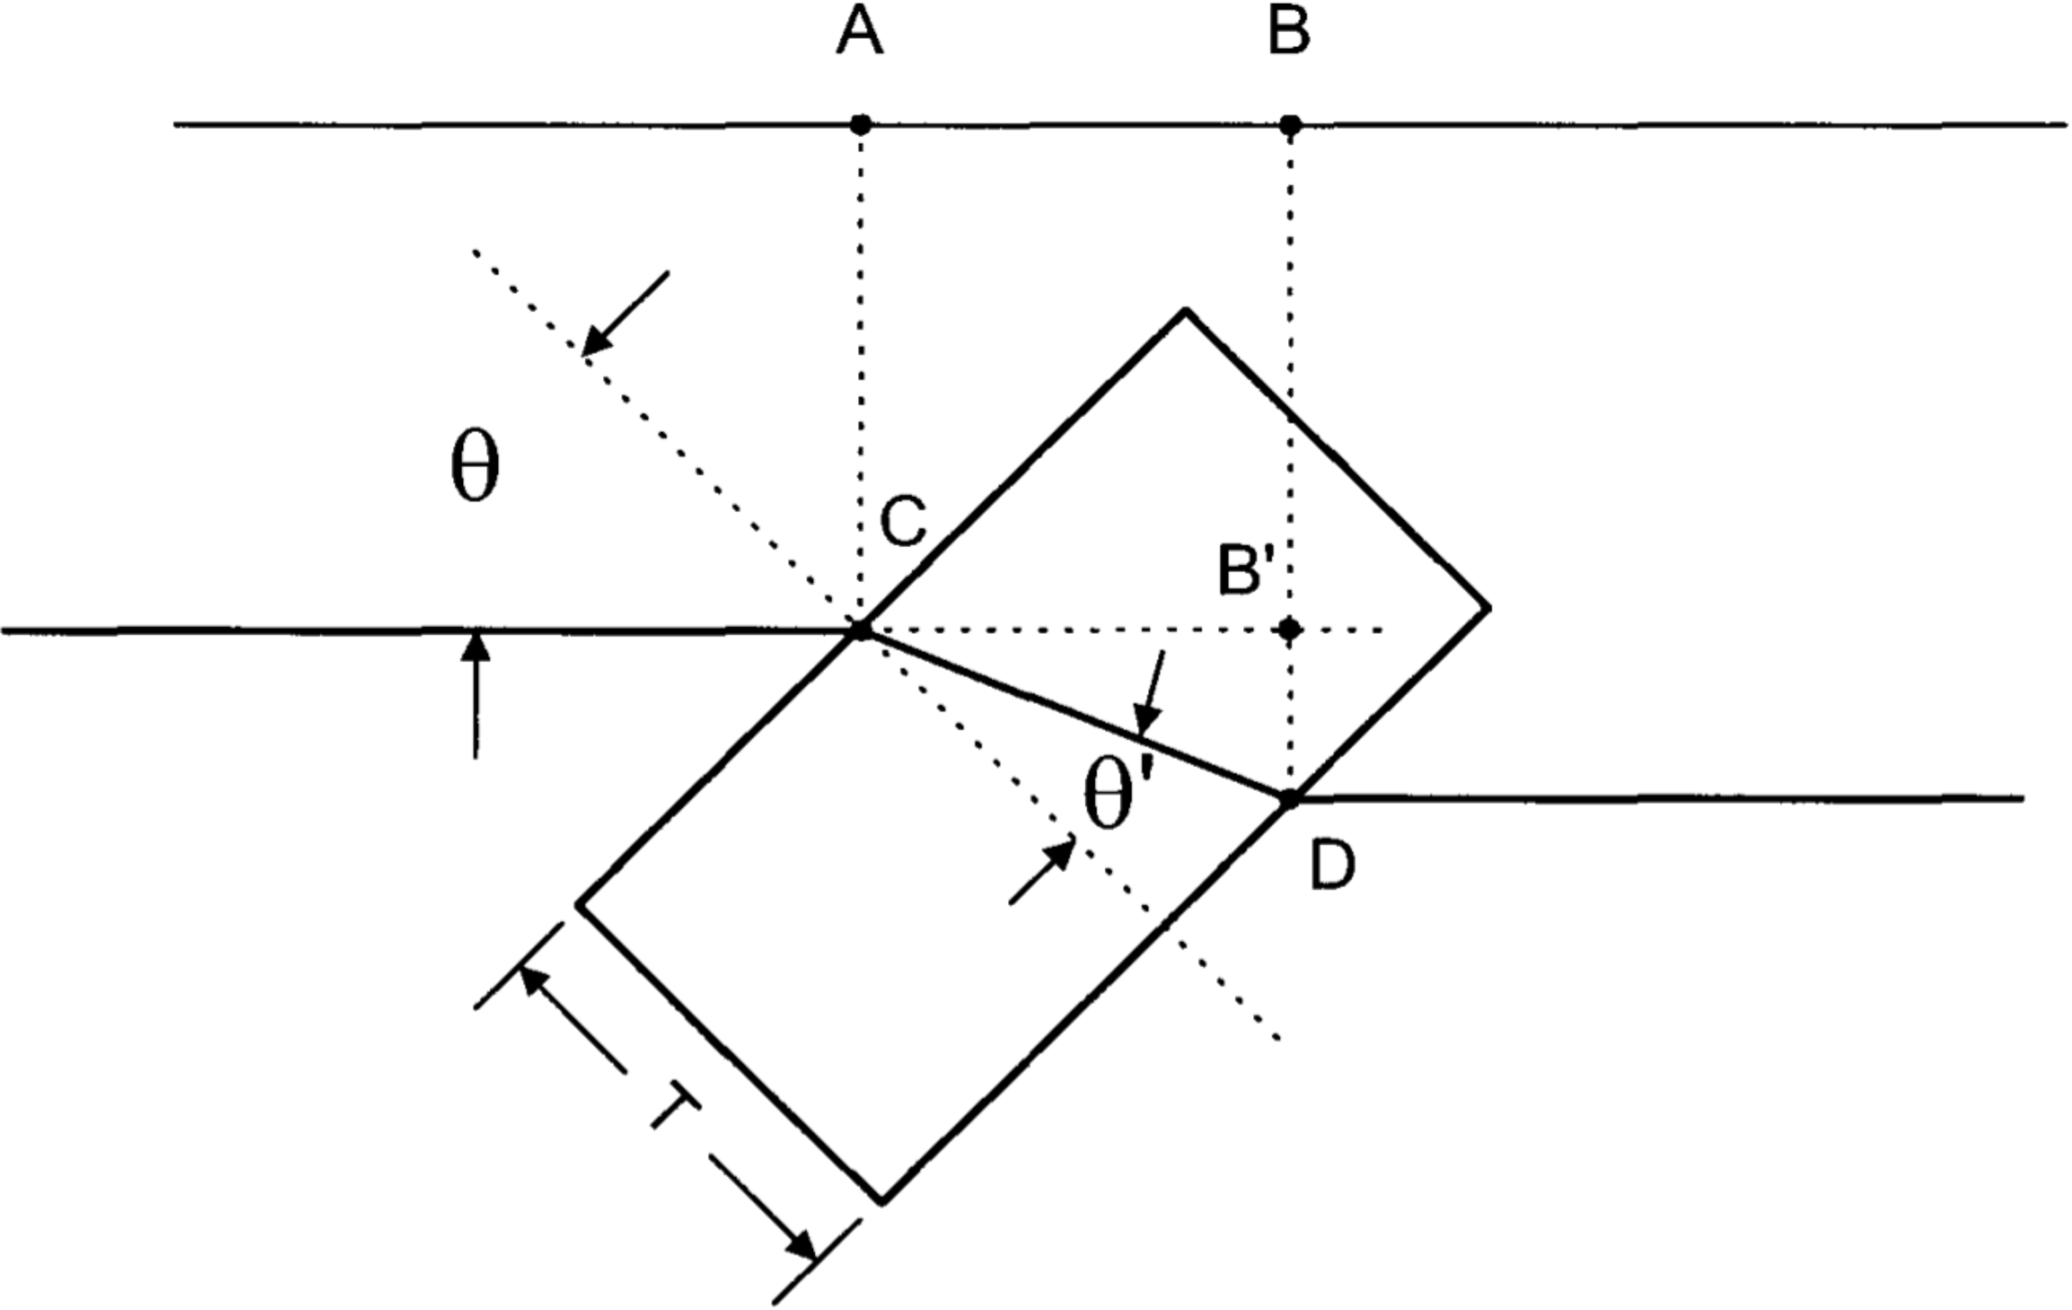
\includegraphics[width=\linewidth]{./figures/glasplaettchen.pdf}
\caption{The geometry of the beam inside a solid medium}
\label{fig:Geometrie}
\end{figure}
A beam of light is refracted when entering a medium. For this reason, the way traveled by the beam that travels through it will be longer than that of the other beam. If the way of the beam outside the medium would be $a$ (between the points A and B, as depicted in \autoref{fig:Geometrie}) and the thickness of the medium be $T$, the way traveled by the beam inside the medium is 
\begin{aquation}
  b &\coloneqq a \cos(\theta^\prime - \theta) \tp
\end{aquation}
With this, the phase difference for a solid body, which can not be determined as easily as with the gas via its pressure and temperature is
\begin{aquation}
\label{eq:phase-difference_solid}
  \Delta \varphi &= \frac{2 \pi}{\lambda_\text{vac}} \lbr n_\text{medium} b - a \rbr \\
  		&=v \frac{2 \pi T}{\lambda_\text{vac}} \lbr \frac{n-\cos(\theta^\prime - \theta)}{\cos(\theta^\prime)}\rbr \tp
\end{aquation}
The angles are related via Snellius' formula
\begin{aquation}
  n \sin(\theta^\prime) &= \sin(\theta) \tp
\end{aquation}
However in this experiment, the medium has been inserted into both beams. It consisted of two glass plates of identical thickness that were mounted on a rotation holder at an angle of $20$ degrees. For this reason, the refraction indices in the above formula become the same, and the formula can be symmetrised. Going through the previous steps again for each beam, at angles $\theta_\pm \coloneqq \theta \pm \theta_0$, with $\theta_0 = 20 \text{degree}$, the final expression for the number of interference maxima is 
\begin{aquation}
  M &= \frac{T}{\lambda_\text{vac}} \lbr \frac{n - \cos\lbr\theta_+ - \arcsin\lbr \frac{\sin(\theta_+)}{n} \rbr\rbr}{\cos\lbr\arcsin\lbr\frac{\sin(\theta_+)}{n}\rbr\rbr} - \frac{n - \cos\lbr\theta_- - \arcsin\lbr \frac{\sin(\theta_-)}{n} \rbr\rbr}{\cos\lbr\arcsin\lbr\frac{\sin(\theta_-)}{n}\rbr\rbr}\rbr
\end{aquation}



